
\documentclass{article}
% pre\'ambulo

\usepackage{lmodern}
\usepackage[T1]{fontenc}
\usepackage[spanish,activeacute]{babel}
\usepackage{enumerate}
\usepackage{graphicx}
\graphicspath{ {/home/nestor2502/Modelado/Tarea01/imagenes/} }

\title{Tarea 01}
\author{Nestor Semer V\'azquez Cordero}
\date{14 de Agosto del a\~no 2019}

\begin{document}
% cuerpo del documento

\maketitle

\section{Definici\'on del problema}

Dar el clima en tiempo real de dos localidades dadas su latitud y longitud, 
usando un web service para poder realizar las multiples peticiones que se requieren.

\section{Analisis del problema}

Tambien se necesita resolver problemas, se consideraran
los siguientes:
\begin{itemize}
 \item El servidor no est\'a disponible
 \item No hay conexi\'on a internet
 \item No se encuentra el archivo en la ruta indicada
 \item El archivo no tiene el formato .csv
 \item No se especifica la ciudad
 \item No se especifica latitud ni longitud
 \end{itemize}

\section{Seccion de la mejor alternativa}

Se utilizar\'a el lenguaje de programacio\'n python ya que es un lenguaje 
lenguaje de alto nivel, 
debido a eso la sintaxis es sencilla, adem\'as  hay librerias que facilitan
 el trabajo al realizar las peticiones y obtener el archivo json.

\section{Diagrama de flujo }
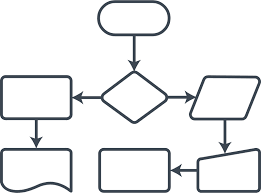
\includegraphics{diagrama}
\section{Pensando en el futuro}

Para este punto se piensa realizar una funci\'on que \'unicamente
reciba como parametros latitud y longitud, as\'i se puede cambiar el servidor, ademas podemos
cambiar los datos que se desean mostrar.



\end{document}
